\graphicspath{{./introduction/}}

\chapter{Introduction}
% {{{
\label{cha:introduction}

Molecular simulations typically generate massive amounts of data. A large
simulation can comprise hundreds of thousands of atoms, with thousands of
frames, yielding many gigabytes of data. Due to the computational costs and
time required to perform these simulations, they are often run on clusters,
which means that the generated data needs to be transferred from the cluster to
a researchers' workstation. Compressing the molecular data is thus advantageous
as it will make transferring the data faster, as well as decreasing the storage
costs.

As water is the solvent in which many molecular simulations occur in, a large
proportion of the volume in these simulations is water. Water has certain
structural properties that can be exploited to achieve good compression ratios.
The water compression project thus targets molecular simulations with large
amounts of water, aiming to achieve high compression ratios by exploiting these
properties.

\section{Overview}
% {{{
\label{sec:introduction_overview}

Molecular simulations are composed of a sequence of frames of data, a single
frame is a snapshot of the positions of all the atoms. Compressing molecular
simulations can thus be broken up into: compressing single frames (intraframe
compression), and compressing data across frames (interframe compression).

Our water compression project has been split into three main parts:

\begin{itemize}
  \item Intraframe compression
  \item Interframe compression
  \item Visualisation
\end{itemize}

The water molecules in a body of water do not group uniformly in all
directions; instead the water molecules form clusters. The presence of these
water clusters are used by the intraframe compressor to perform prediction, and
thus compression.

The interframe compression is more general, it compresses all the atom
information, water and non-water molecules. Using previous frames of data, the
position of atoms in the next frame are predicted, and the errors are encoded.

The visualisation component of the project supports the main goal of the project:
compressing molecular simulations. To do so, the molecular simulation data will
need to be visualised, and a quantisation experiment carried out. Section
\ref{sec:introduction_quantisation} introduces and explains the need for the
quantisation experiment. Section \ref{sec:introduction_visualisation}
introduces the visualisation infrastructure developed for the quantisation
experiment.

This report focuses on the visualisation component of the water compression
project. The intraframe and interframe components of the system are handled in
their respective reports.

% }}}

\section{Quantisation Experiment}
% {{{
\label{sec:introduction_quantisation}

Quantisation maps floating point values onto integer values, ranges of floating
point values are mapped to different integer values. Quantising point data
will have the effect of snapping the points to a grid. Figure
\ref{fig:introduction_quantisation} illustrates the effects of quantisation;
unquantised points are shown in the left image, the quantised points are in the
right image.

\begin{figure}
  \begin{center}
    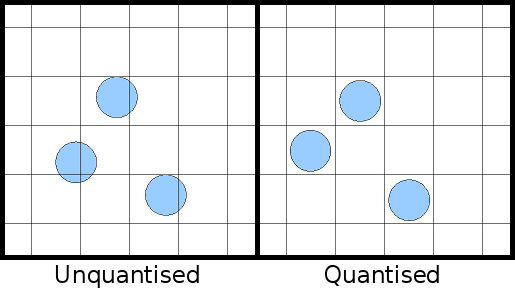
\includegraphics[width=100mm]{quantisation}
  \end{center}
  \caption{Diagram showing unquantised points (left) and quantised points
  (right).}
  \label{fig:introduction_quantisation}
\end{figure}

Quantisation is used to facilitate compressing the molecular data, integer
values can be more effectively compressed than floating point values.
Quantisation using fewer bits will increase the compression ratio as there will
be fewer distinct values to encode, but fewer distinct values will result in
greater deviation from the original data. Quantisation is the only lossy step
in the compression process, the following steps in the compression process are
all lossless, no data is discarded.

With quantisation, a balance needs to be established between data fidelity and
compression ratio. Determining this balance is the aim of the quantisation
experiment: what is an acceptable level of quantisation? The acceptable level
of quantisation is where the differences between the original and quantised
data are not significantly noticeable.

% }}}

\section{Visualisation}
% {{{
\label{sec:introduction_visualisation}

The other aspect to the visualisation component of the system is to provide
visualisations of the molecular data. The visualisations used in the
quantisation experiment supports the compression components of the system, and
can be used for simple molecular data visualisation.

Due to the specific uses that are needed by the project, an existing
visualisation package is insufficient. Specific visualisations such as showing
the water clusters used by the intraframe compressor, or quantisation errors
are not present in existing packages. A separate visualisation component is
thus developed to provide the infrastructure needed for the quantisation
experiment, as well as provide the compression specific visualisations.

% }}}

\section{Outline}
% {{{
\label{sec:introduction_outline}

The remainder of this report is structured as follows:

Chapter \ref{cha:background} provides background on relevant visualisation
techniques that influenced the development of our visualisation.

Chapter \ref{cha:design} identifies and details a number of visualisation
solutions. The chapter explains why these approaches are chosen and the design
behind them. A few of the visualisation approaches are aimed purely at
supporting the compressors.

Chapter \ref{cha:implementation} provides implementation details on each of the
visualisation components.

Chapter \ref{cha:experiment} details the quantisation experiment.

Chapter \ref{cha:results} contains the experiment results and analysis.

Finally, Chapter \ref{cha:conclusion} concludes and summarises this report.

% }}}

% }}}

